\documentclass[tikz, margin=3mm]{standalone}
\usepackage{tikz}
\begin{document}
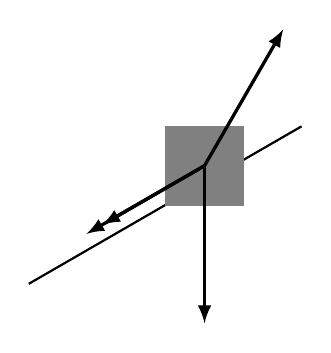
\begin{tikzpicture}
    % Draw incline
    \draw[thick] (0,0) -- (30:4);
    % Draw block
    \filldraw[gray] (30:2) rectangle ++(1,1);
    % Draw forces
    % Weight
    \draw[very thick, -latex] (30:2) ++(0.5,0.5) -- ++(0,-2);
    % Normal force
    \draw[very thick, -latex] (30:2) ++(0.5,0.5) -- ++(60:2);
    % Friction
    \draw[very thick, -latex] (30:2) ++(0.5,0.5) -- ++(210:1.5);
    % Component of weight parallel to incline
    \draw[very thick, -latex] (30:2) ++(0.5,0.5) -- ++(30:-1.732);
\end{tikzpicture}
\end{document}